% Copyright 2004 by Till Tantau <tantau@users.sourceforge.net>.
%
% In principle, this file can be redistributed and/or modified under
% the terms of the GNU Public License, version 2.
%
% However, this file is supposed to be a template to be modified
% for your own needs. For this reason, if you use this file as a
% template and not specifically distribute it as part of a another
% package/program, I grant the extra permission to freely copy and
% modify this file as you see fit and even to delete this copyright
% notice. 

\documentclass[xcolor=table]{beamer}
\usepackage{menukeys}[os=win]
\usepackage{textcomp}
\usepackage{tcolorbox}
\usepackage{lmodern}
\usepackage{listings}
\lstset{
  basicstyle=\tiny\ttfamily,
}

% There are many different themes available for Beamer. A comprehensive
% list with examples is given here:
% http://deic.uab.es/~iblanes/beamer_gallery/index_by_theme.html
% You can uncomment the themes below if you would like to use a different
% one:
%\usetheme{AnnArbor}
%\usetheme{Antibes}
%\usetheme{Bergen}
%\usetheme{Berkeley}
%\usetheme{Berlin}
%\usetheme{Boadilla}
%\usetheme{boxes}
%\usetheme{CambridgeUS}
%\usetheme{Copenhagen}
%\usetheme{Darmstadt}
%\usetheme{default}
%\usetheme{Frankfurt}
%\usetheme{Goettingen}
%\usetheme{Hannover}
%\usetheme{Ilmenau}
\usetheme{JuanLesPins}
%\usetheme{Luebeck}
%\usetheme{Madrid}
%\usetheme{Malmoe}
%\usetheme{Marburg}
%\usetheme{Montpellier}
%\usetheme{PaloAlto}
%\usetheme{Pittsburgh}
%\usetheme{Rochester}
%\usetheme{Singapore}
%\usetheme{Szeged}
%\usetheme{Warsaw}
\setbeamerfont{block body}{size=\small}
\title{KF5004 - Apache}
\titlegraphic{
\includegraphics[width=0.3\textwidth]{../images/logo.png}}


% A subtitle is optional and this may be deleted
% \subtitle{(Using proximity detection)}

\author{Dr.~Neil~Eliot \& Dr.~Alun~Moon}
% - Give the names in the same order as the appear in the paper.
% - Use the \inst{?} command only if the authors have different
%   affiliation.

%\renewcommand\appendixname{Appendix}

\institute[Northumbria University] % (optional, but mostly needed)
{
  Department of Computer and Information Sciences\\
  University of Northumbria
  % \and
  % \inst{2}
  % Department of Theoretical Philosophy\\
  % University of Elsewhere
}
% - Use the \inst command only if there are several affiliations.
% - Keep it simple, no one is interested in your street address.

\date{Session 8}
% - Either use conference name or its abbreviation.
% - Not really informative to the audience, more for people (including
%   yourself) who are reading the slides online

\subject{Introduction}
% This is only inserted into the PDF information catalog. Can be left
% out. 

% If you have a file called "university-logo-filename.xxx", where xxx
% is a graphic format that can be processed by latex or pdflatex,
% resp., then you can add a logo as follows:

% \pgfdeclareimage[height=0.5cm]{university-logo}{university-logo-filename}
% \logo{\pgfuseimage{university-logo}}

% Delete this, if you do not want the table of contents to pop up at
% the beginning of each subsection:
% \AtBeginSubsection[]
% {
%   \begin{frame}<beamer>{Outline}
%     \tableofcontents[currentsection,currentsubsection]
%   \end{frame}
% }

% Let's get started

\begin{document}

\begin{frame}
  \titlepage
\end{frame}

\begin{frame}{Introduction}
  \tableofcontents
  % You might wish to add the option [pausesections]
\end{frame}

% Section and subsections will appear in the presentation overview
% and table of contents.

\section{Introduction}
\subsection{Background}
\begin{frame}{Why \texttt{Apache}?}
    \begin{figure}
      \begin{center}
        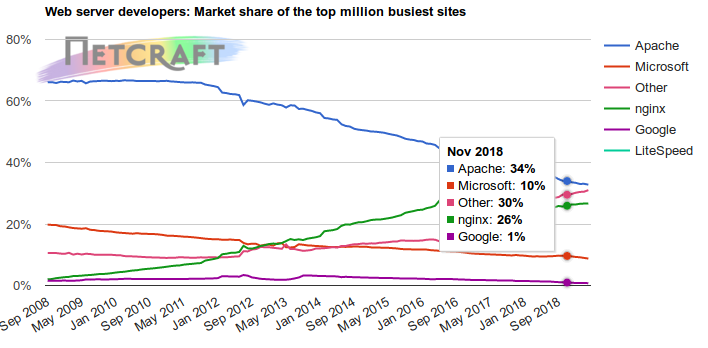
\includegraphics[width=1\linewidth]{Market.png}
      \end{center}
    \end{figure}
\end{frame}

\begin{frame}{What is a Webserver?}
  \begin{figure}
    \begin{center}
      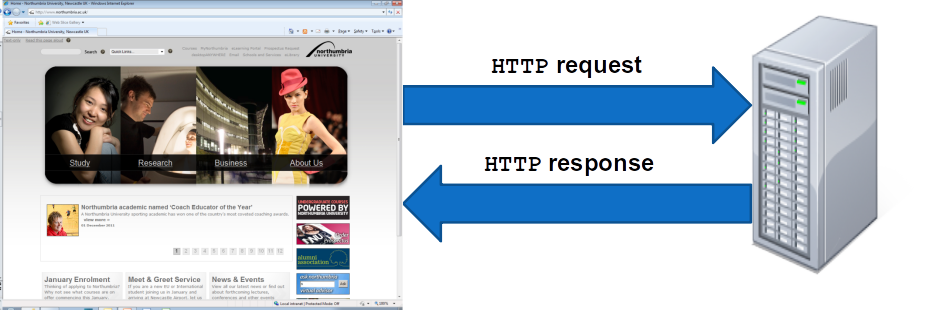
\includegraphics[width=1\linewidth]{What.png}
    \end{center}
  \end{figure}
\end{frame}

\section{\texttt{HTTP}}
\subsection{\texttt{HEADERS}}
\begin{frame}{Connections?}
  \begin{itemize}
    \item There are two ways to connect to a webserver.
      \begin{itemize}
        \item Via a \texttt{URL} lookup.
        \item Directly using an \texttt{IP} Address
      \end{itemize}
    \item The \texttt{HTTP} request header varies based on the route.
  \end{itemize}
\end{frame}

\begin{frame}[fragile]{Via a \texttt{URL}}
  \begin{itemize}
      \item \texttt{URL} Based Transaction
      \begin{itemize}
        \item \texttt{DNS} Query
        \item \texttt{DNS} Response
          \begin{itemize}
            \item Client now has both a \texttt{URL} and an \texttt{IP} Address for the server.
          \end{itemize}
      \end{itemize}
      \begin{center}
        e.g. \texttt{URL} \texttt{www.offcampusnetwork.co.uk}        
      \end{center}
    \end{itemize}
  \begin{tcolorbox}
    \lstset{
      basicstyle=\tiny\ttfamily,
    }
    \begin{lstlisting}
      GET / HTTP/1.1
      Accept: image/jpeg, application/x-ms-application, image/gif, */*
      Accept-Language: en-GB
      User-Agent: Mozilla/4.0 (compatible; MSIE 8.0; Windows NT 6.1; ....)
      Accept-Encoding: gzip, deflate
      Host: www.offcampusnetwork.co.uk
      Connection: Keep-Alive
    \end{lstlisting}
  \end{tcolorbox}
\end{frame}

\begin{frame}[fragile]{Via an \texttt{IP} Address}
  \begin{itemize}
      \item \texttt{IP} Based Transaction
        \begin{itemize}
          \item Client has only an \texttt{IP} Address for the server.
        \end{itemize}
      \begin{center}
        e.g. \texttt{IP} \texttt{192.168.101.249}        
      \end{center}
    \end{itemize}
  \begin{tcolorbox}
    \lstset{
      basicstyle=\tiny\ttfamily,
    }
    \begin{lstlisting}
      GET / HTTP/1.1
      Accept: image/jpeg, application/x-ms-application, image/gif, */*
      Accept-Language: en-GB
      User-Agent: Mozilla/4.0 (compatible; MSIE 8.0; Windows NT 6.1; ....)
      Accept-Encoding: gzip, deflate
      Host: 192.168.101.249
      Connection: Keep-Alive
    \end{lstlisting}
  \end{tcolorbox}
\end{frame}

\section{\texttt{Apache2}}
\begin{frame}{Why \texttt{Apache}?}
  \begin{itemize}
    \item \texttt{Apache} is the most commonly used Web Server on \texttt{Linux} systems and the Internet.
      \begin{itemize}
        \item Top 1 Million sites (NETCRAFT 2019).
      \end{itemize}
    \item \texttt{Apache} Web Servers are often used in combination with a \texttt{MySQL/MariaDB} database engine (Later!)
    \item \texttt{Apache} supports dynamic applications using the HyperText Preprocessor (\texttt{PHP}) scripting language. 
      \begin{itemize}
        \item Other popular scripting languages such as \texttt{Python} and \texttt{Perl}.
      \end{itemize}
  \end{itemize}
  \begin{tcolorbox}
    \begin{center}
      \scriptsize This configuration is referred to as a \texttt{LAMP} installation (\texttt{Linux, Apache, MySQL and Perl/Python/PHP})
    \end{center}
  \end{tcolorbox}
\end{frame}

\subsection{Installation}
\begin{frame}[fragile]{Installing \texttt{Apache}}
  \begin{tcolorbox}
    \begin{center}
      \scriptsize \texttt{\$sudo apt-get install apache2}
    \end{center}
  \end{tcolorbox}
  \begin{tcolorbox}
    \lstset{
      basicstyle=\tiny\ttfamily,
    }
    \begin{lstlisting}
    Reading package lists... Done
    Building dependency tree
    Reading state information... Done
    Preparing to unpack .../apache2_2.4.29-1ubuntu4.1_amd64.deb ...
    Unpacking apache2 (2.4.29-1ubuntu4.1) ...
    Processing triggers for ufw (0.35-5) ...
    Setting up apache2 (2.4.29-1ubuntu4.1) ...
    Enabling module mpm_event.
    Enabling module authz_core.
    Created symlink /etc/systemd/system/multi-user.target.wants ...
    Created symlink /etc/systemd/system/multi-user.target.wants ...
    Processing triggers for ureadahead (0.100.0-20) ...
    Processing triggers for systemd (237-3ubuntu10) ...
    Processing triggers for man-db (2.8.3-2) ...
    Processing triggers for ufw (0.35-5) ...
    student@a123456789:~$
    \end{lstlisting}
  \end{tcolorbox}
\end{frame}

\begin{frame}{Installation Done}
  \begin{itemize}
    \item You now have a basic \texttt{Apache} installation supporting a basic \texttt{HTML} website.
  \end{itemize}
  \begin{figure}
    \begin{center}
      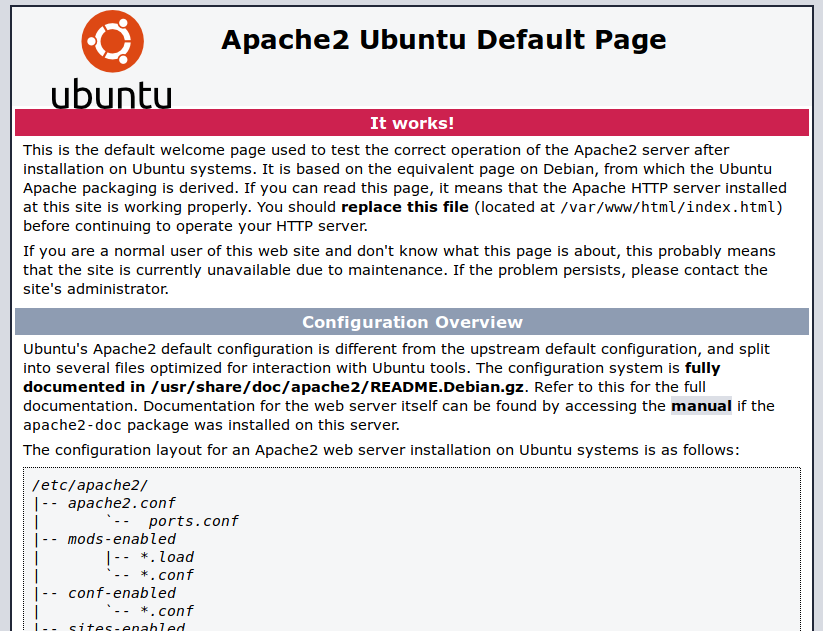
\includegraphics[width=0.6\linewidth]{IntroPage.png}
    \end{center}
  \end{figure}
\end{frame}

\begin{frame}[fragile]{Apache Configuration}
  \begin{itemize}
    \item \texttt{apache2.conf}
      \begin{itemize}
        \item The main \texttt{Apache2} configuration file. 
        \item Contains settings that are global to \texttt{Apache2}.
      \end{itemize}
  \end{itemize}
  \begin{tcolorbox}
    \lstset{
      basicstyle=\tiny\ttfamily,
    }
    \begin{lstlisting}
      # This is the main Apache server configuration file.  
      # It contains the configuration directives that give the 
      # server its instructions.
      # See http://httpd.apache.org/docs/2.4/ for detailed information 
      # about the directives and /usr/share/doc/apache2/README.Debian 
      # about Debian specific hints.
      ...
    \end{lstlisting}
  \end{tcolorbox}
\end{frame}

\subsection{Configuration}
\begin{frame}[fragile]{\texttt{Apache} Configuration}
  \begin{itemize}
    \item \texttt{Apache2} is configured by placing directives in plain text configuration files. 
    \item These directives are separated between files and directories
  \end{itemize}
  \begin{tcolorbox}
    \lstset{
      basicstyle=\tiny\ttfamily,
    }
    \begin{lstlisting}
      student@a123456789:~$ cd /etc/apache2
      student@a123456789:/etc/apache2$ ls
      apache2.conf    magic           sites-available
      conf-available  mods-available  sites-enabled
      conf-enabled    mods-enabled
      envvars         ports.conf
      student@a123456789:/etc/apache2$
    \end{lstlisting}
  \end{tcolorbox}
\end{frame}

\begin{frame}{\texttt{Apache} Configuration}
  \begin{itemize}
    \item Configuration directories.
      \begin{itemize}
        \item \texttt{sites-available}
        \item \texttt{conf-available}  
        \item \texttt{mods-available}  
        \item \texttt{sites-enabled}
        \item \texttt{conf-enabled}    
        \item \texttt{mods-enabled}
      \end{itemize}
  \end{itemize}
\end{frame}

\begin{frame}{\texttt{Apache} Configuration}
  \begin{itemize}
    \item \texttt{envars}
      \begin{itemize}
        \item This file is where \texttt{Apache2} environment variables are set.
        \item The file is a script file and can therefore contain logic and also executable commands.
        \item Dynamic website contain scripts that can create files and directories.
          \begin{itemize} 
            \item \texttt{PHP}
          \end{itemize}
        \item Default options for files and directories can be set when the server creates them.
          \begin{itemize} 
            \item \texttt{umask}
          \end{itemize}
      \end{itemize}
  \end{itemize}
\end{frame}

\begin{frame}[fragile]{\texttt{Apache} Configuration}
  \begin{itemize}
    \item \texttt{envars}
  \end{itemize}
  \begin{tcolorbox}
    \lstset{
      basicstyle=\tiny\ttfamily,
    }
    \begin{lstlisting}
      # envvars - default environment variables for apache2ctl
      unset HOME
      if [ "${APACHE_CONFDIR##/etc/apache2-}" != "${APACHE_CONFDIR}" ] ; then
        SUFFIX="-${APACHE_CONFDIR##/etc/apache2-}"
      else
        SUFFIX=
      fi
      export APACHE_RUN_USER=www-data
      export APACHE_RUN_GROUP=www-data
      export APACHE_PID_FILE=/var/run/apache2/apache2$SUFFIX.pid
      export APACHE_RUN_DIR=/var/run/apache2$SUFFIX
      export APACHE_LOCK_DIR=/var/lock/apache2$SUFFIX
      export APACHE_LOG_DIR=/var/log/apache2$SUFFIX
      export LANG=C
      export LANG
      #export APACHE_LYNX='www-browser -dump'
      #APACHE_ULIMIT_MAX_FILES='ulimit -n 65536'
      #export APACHE_ARGUMENTS=''
      #export APACHE2_MAINTSCRIPT_DEBUG=1
      umask 002
    \end{lstlisting}
  \end{tcolorbox}
\end{frame}

\begin{frame}{\texttt{Apache} Configuration}
  \begin{itemize}
    \item \texttt{mods-available}
      \begin{itemize}
        \item This directory contains configuration files to both load modules and configure them. 
        \item Not all modules will have specific configuration files.
      \end{itemize}
  \end{itemize}
\end{frame}

\begin{frame}{\texttt{Apache} Configuration}
  \begin{itemize}
    \item This directory holds \texttt{symlinks} to the files in \texttt{/etc/apache2/mods-available}. 
      \begin{itemize}
        \item Created by \texttt{a2enmod}
      \end{itemize}
    \item When a module configuration file is \textit{``symlinked''} it will be enabled the next time \texttt{apache2} is restarted.
  \end{itemize}
\end{frame}

\begin{frame}{\texttt{Apache} Configuration}
  \begin{itemize}
    \item \texttt{ports.conf} 
      \begin{itemize}
        \item This file contains the directives that determine which \texttt{TCP} ports \texttt{Apache2} is listening on.
        \item \texttt{Apache2} can listen on more than one port at a time and can also listen for the same \texttt{URL} on different ports.
        \item Common ports for development and beta sites.
          \begin{itemize}
            \item \texttt{8080}
            \item \texttt{81}
          \end{itemize}
      \end{itemize}
  \end{itemize}
\end{frame}

\begin{frame}[fragile]{\texttt{Apache} Configuration}
  \begin{itemize}
    \item \texttt{ports.conf}
  \end{itemize}
  \begin{tcolorbox}
    \lstset{
      basicstyle=\tiny\ttfamily,
    }
    \begin{lstlisting}
      # If you just change the port or add more ports 
      # you have to change the VirtualHost statement in
      # /etc/apache2/sites-enabled/000-default.conf

      Listen 80

      <IfModule ssl_module>
          Listen 443
      </IfModule>

      Listen 8080
      Listen 81
    \end{lstlisting}
  \end{tcolorbox}
\end{frame}

\begin{frame}{\texttt{Apache} Configuration}
  \begin{itemize}
    \item \texttt{sites-available} 
      \begin{itemize}
        \item This directory has configuration files for \texttt{Apache2 Virtual Hosts}. 
        \item \texttt{Virtual Hosts} allow a single copy of \texttt{Apache2} to be configured for multiple sites that have separate configurations.
      \end{itemize}
  \end{itemize}
\end{frame}

\begin{frame}{\texttt{Apache} Configuration}
  \begin{itemize}
    \item \texttt{sites-enabled} 
      \begin{itemize}
        \item Like \texttt{mods-enabled, sites-enabled} contains \textit{symlinks}.  \texttt{sites-enabled} contains \textit{symlinks} to the files in \texttt{/etc/apache2/sites-available} directory. 
        \item The site will be active once \texttt{Apache2} is restarted.
          \begin{itemize}
            \item \texttt{a2ensite \textless filename\textgreater}
            \item \texttt{a2dissite \textless filename\textgreater}
          \end{itemize}
      \end{itemize}
  \end{itemize}
\end{frame}

\begin{frame}{\texttt{Apache} Configuration}
  \begin{itemize}
    \item \texttt{Apache2} ships with a virtual-host-friendly default configuration. 
      \begin{itemize}
        \item The default site is located in \texttt{/var/www/html}
      \end{itemize}
    \item It is configured with a single default \texttt{virtual host} (using the \texttt{VirtualHost} directive) which can be modified or used as-is if you have a single site.
      \begin{itemize}
        \item It can be used as a template for additional \texttt{virtual hosts} if you require multiple sites. 
      \end{itemize}
  \end{itemize}
\end{frame}

\begin{frame}{\texttt{Apache} Configuration}
  \begin{itemize}
    \item The default \texttt{virtual host} will serve as the site users will see if the \texttt{URL} they enter does not match the \texttt{ServerName} directive of any of your custom sites or they enter an \texttt{IP} address. 
    \item To modify the default \texttt{virtual host} edit:
      \begin{itemize}
        \item \texttt{/etc/apache2/sites-available/000-default.conf}
      \end{itemize}
  \end{itemize}
  \begin{tcolorbox}
    \begin{center}
      \scriptsize The \texttt{ServerName} is obtained from the \texttt{HTTP Header}'s \texttt{host:} directive.
    \end{center}
  \end{tcolorbox}
\end{frame}

\begin{frame}{\texttt{Apache} Configuration}
  \begin{itemize}
    \item Multi website support:
      \begin{itemize}
        \item \texttt{Virtual Hosts}
        \item \texttt{User-based}
      \end{itemize}
  \end{itemize}
  \begin{tcolorbox}
    \begin{center}
      \scriptsize This module will only cover \texttt{User-based} multi-website support and using the \texttt{default} site.
    \end{center}
  \end{tcolorbox}
\end{frame}

\subsection{Large Corporate website support}
\begin{frame}{\texttt{Apache} Configuration - Load-balancing}
  \begin{itemize}
    \item The default \texttt{virtual host} set-up provides a single website.
    \item A \texttt{DNS} Server can resolve a \texttt{domain name} to multiple \texttt{IP} addresses.
    \item Most modern web browsers will use the \texttt{IP} addresses in sequence until one of the servers responds.
    \item Once a functioning \texttt{IP} address is resolved the browser will return to that address.
  \end{itemize}
  \begin{tcolorbox}
    \begin{center}
      \scriptsize In effect we are able to have a single \texttt{URL} being supported by several servers.
    \end{center}
  \end{tcolorbox}
\end{frame}

\begin{frame}{\texttt{Apache} Configuration - Load-balancing}
  \begin{figure}
    \begin{center}
      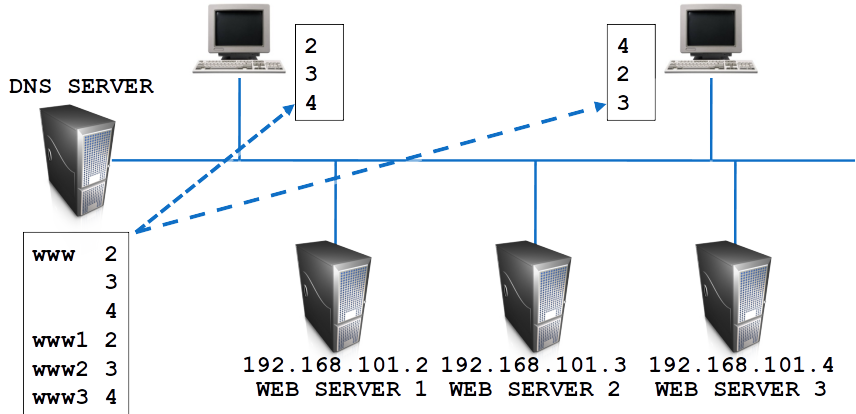
\includegraphics[width=1\linewidth]{LoadBalanced.png}
    \end{center}
  \end{figure}
\end{frame}

\begin{frame}[fragile]{\texttt{bind9} and Load-balancing}
  \begin{itemize}
    \item \texttt{bind9} supports load-balancing by providing multiple \texttt{IP} addresses for a single \texttt{URL}
    \item The \texttt{name} component of the \texttt{bind9} entry can consist of \texttt{A} and \texttt{AAAA} records.
  \end{itemize}
  \begin{tcolorbox}
    \begin{center}
      \scriptsize This module will only use \texttt{A} records (\texttt{IPv4}).
    \end{center}
  \end{tcolorbox}
  \begin{columns}
    \begin{column}{0.5\textwidth}
      \begin{tcolorbox}
        \lstset{
          basicstyle=\scriptsize\ttfamily,
        }
    \begin{lstlisting}
  ...
www IN   192.168.101.2
    IN	 192.168.101.3
    IN	 192.168.101.4
  ...
    \end{lstlisting}
      \end{tcolorbox}
    \end{column}
    \begin{column}{0.5\textwidth}
      \begin{tcolorbox}
        \lstset{
          basicstyle=\scriptsize\ttfamily,
        }
    \begin{lstlisting}
  ...
www IN   192.168.101.2
www IN   192.168.101.3
www IN   192.168.101.4
  ...
    \end{lstlisting}
      \end{tcolorbox}
    \end{column}
  \end{columns}
\end{frame}

\begin{frame}{\texttt{bind9} and Load-balancing}
  \begin{itemize}
    \item \texttt{bind9} supports \textit{round robin} and \textit{random} selection of records by allowing the order of any duplicate records (\texttt{names}) to be sequenced.
    \item Sequencing can be specified on a \texttt{zone} basis or globally.
  \end{itemize}
  \begin{figure}
    \begin{center}
      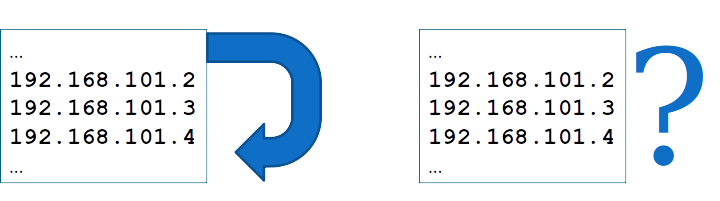
\includegraphics[width=1\linewidth]{rrset.png}
    \end{center}
  \end{figure}
\end{frame}

\begin{frame}[fragile]{\texttt{bind9} and Load-balancing}
  \begin{itemize}
    \item Global sequencing is achieved by making an entry in the \texttt{named.conf.options} file.
  \end{itemize}
  \begin{columns}
    \begin{column}{0.5\textwidth}
      \begin{tcolorbox}
        \lstset{
          basicstyle=\scriptsize\ttfamily,
        }
    \begin{lstlisting}
options {
  ...
  rrset-order {
      order cyclic;
      ...
      };
};
    \end{lstlisting}
      \end{tcolorbox}
    \end{column}
    \begin{column}{0.5\textwidth}
      \begin{tcolorbox}
        \lstset{
          basicstyle=\scriptsize\ttfamily,
        }
    \begin{lstlisting}
options {
  ...
  rrset-order {
    order random;
  };
  ...
};
    \end{lstlisting}
      \end{tcolorbox}
    \end{column}
  \end{columns}
\end{frame}

\subsection{Managing the \texttt{Apache2 daemon}}
\begin{frame}{\texttt{Apache2} Starting/Stopping}
  \begin{itemize}
    \item The \texttt{Apache2 daemon} can be controlled by the \texttt{systemctl} command.
      \begin{itemize}
        \item \texttt{\$sudo systemctl start apache2}
        \item \texttt{\$sudo systemctl stop apache2}
      \end{itemize}
  \end{itemize}
  \begin{tcolorbox}
    \begin{center}
      \scriptsize \textbf{Although this seems like a logical approach you should be VERY CAUTIOUS of using this technique! It causes \texttt{Apache} to stop abruptly and can damage data transactions in a web application.}
    \end{center}
  \end{tcolorbox}
\end{frame}

\begin{frame}{\texttt{Apache2} Starting/Stopping}
  \begin{itemize}
    \item There is a tool specifically designed to control \texttt{Apache2}.
      \begin{itemize}
        \item \texttt{apachectl}
      \end{itemize}
    \item To forcefully terminate \texttt{Apache2} and any transactions.
      \begin{itemize}
        \item \texttt{\$sudo apachectl -k stop}
      \end{itemize}
    \item To gracefully allow all transactions to complete before shutting down the \texttt{daemons}. 
      \begin{itemize}
        \item \texttt{\$sudo apachectl -k graceful-stop}
      \end{itemize}
    \item To restart \texttt{Apache}
      \begin{itemize}
        \item \texttt{\$sudo apachectl -k start}
      \end{itemize}
  \end{itemize}
  \begin{tcolorbox}
    \begin{center}
      \scriptsize \textbf{These commands are the prefered way to control \texttt{Apache} to ensure data integrity with dynamic web applications is maintained.}
    \end{center}
  \end{tcolorbox}
\end{frame}

\begin{frame}{\texttt{Apache2} Starting/Stopping}
  \begin{itemize}
    \item Configuration changes are implemented by restarting \texttt{Apache2}.
      \begin{itemize}
        \item A graceful restart allows all current transactions to be completed. 
        \item Restarting the parent process (\texttt{httpd}) re-reads the configuration files and re-opens the log files. As each child dies off the parent replaces it with a child from the new generation of the configuration. This process begins serving new requests immediately.
          \begin{itemize}
            \item Users don't see the service stopping and availability is maintained.
            \item \texttt{\$sudo apachectl -k graceful}
          \end{itemize}
      \end{itemize}
    \end{itemize}
\end{frame}

\begin{frame}{\texttt{Apache2} enabling/disabling modules}
  \begin{itemize}
    \item Most features are available as modules:
      \begin{itemize}
        \item \texttt{PHP} support
        \item \texttt{MySQL} Authentication support
        \item \texttt{Per-User} Website support
      \end{itemize}
    \item The \texttt{Apache Foundation} has gone some way to automating the process by implementing some additional commands.
  \end{itemize}
\end{frame}

\begin{frame}{\texttt{Apache2} enabling/disabling modules}
  \begin{itemize}
    \item Enabling - \texttt{a2enmod}
      \begin{itemize}
        \item This command simply adds a symbolic link to the \texttt{/etc/apache2/mods-available} directory.
          \begin{itemize}
            \item \texttt{\$sudo a2enmod php}
          \end{itemize}
        \end{itemize}
    \item Disabling - \texttt{a2dismod}
        \begin{itemize}
          \item This command simply removes a symbolic link from the \texttt{/etc/apache2/mods-available} directory.
            \begin{itemize}
              \item \texttt{\$sudo a2dismod php}
            \end{itemize}
          \end{itemize}
    \item Enabling and disabling requires an \texttt{apache2} restart for it to take effect.
  \end{itemize}
\end{frame}

\subsection{Adding multi-website features}
\begin{frame}{Enabling \texttt{Per-User} Websites}
   \begin{itemize}
      \item Step 1 - Enabling - Per-User
        \begin{itemize}
          \item \texttt{\$sudo a2enmod userdir}
        \end{itemize}
      \item  Step 2 - Configure the \texttt{users} home directory.
        \begin{itemize}
          \item \texttt{\$mkdir public\_html} 
          \item \texttt{\$chmod 755 public\_html}
        \end{itemize}
        \begin{tcolorbox}
          \begin{center}
            \scriptsize \textbf{The last two commands should be executed by the user in their home directory.}
          \end{center}
        \end{tcolorbox}
      \item  Step 3 - Add \texttt{HTML} files to the \texttt{public\_html} folder.
    \end{itemize}
\end{frame}

\begin{frame}{Enabling \texttt{Per-User} Websites}
  \begin{itemize}
     \item Step 4 - Restart \texttt{Apache}
       \begin{itemize}
         \item \texttt{\$sudo apachectl -k graceful}
       \end{itemize}
     \item  Step 5 - Access the user website.
       \begin{itemize}
         \item Enter the \texttt{URL} for the site and append the name with a tilde (\texttt{\textasciitilde}) and the \texttt{username}. 
       \end{itemize}
   \end{itemize}
   \begin{tcolorbox}
    \begin{center}
      \scriptsize e.g. For user \texttt{student} on \texttt{domain www.student.co.uk}\\\texttt{http://www.student.co.uk/\textasciitilde student}
    \end{center}
  \end{tcolorbox}
\end{frame}

\subsection{Dynamic websites (\texttt{PHP})}
\begin{frame}{Enabling \texttt{PHP} Websites}
   \begin{itemize}
      \item Install \texttt{PHP}
        \begin{itemize}
          \item \texttt{\$sudo apt-get install php}
          \item \texttt{\$sudo apt-get install libapache2-mod-php}
          \item \texttt{\$sudo apt-get install php-mysql}
          \item \texttt{\$sudo a2enmod php7.2}
          \item \texttt{\$sudo apachectl -k graceful}
            \begin{tcolorbox}
              \begin{center}
                 \scriptsize \textbf{At time of writing \texttt{php7.2} is correct but this may change.}
              \end{center}
            \end{tcolorbox}
        \end{itemize}
    \end{itemize}
    \begin{tcolorbox}
      \begin{center}
        \scriptsize \textbf{\texttt{PHP} can also be used as a command line scripting environment.}
      \end{center}
    \end{tcolorbox}
\end{frame}

\begin{frame}[fragile]{Testing \texttt{PHP}}
  \begin{itemize}
     \item To identify the \texttt{PHP} version information.
       \begin{itemize}
         \item \texttt{\$php -v}
       \end{itemize}
    \item You can test the \texttt{Apache2} installation by creating a simple information page (\texttt{info.php}) in \texttt{/var/www/html} and accessing it via a browser.
      \begin{itemize}
        \item \texttt{https://www.student.co.uk/info.php}
      \end{itemize}
  \end{itemize}
  \begin{tcolorbox}
    \lstset{
      basicstyle=\scriptsize\ttfamily,
    }
\begin{lstlisting}
                    <?php 
                        phpinfo(); 
                    ?>
\end{lstlisting}
  \end{tcolorbox}
\end{frame}

\begin{frame}{Testing \texttt{PHP}}
  \begin{figure}
    \begin{center}
      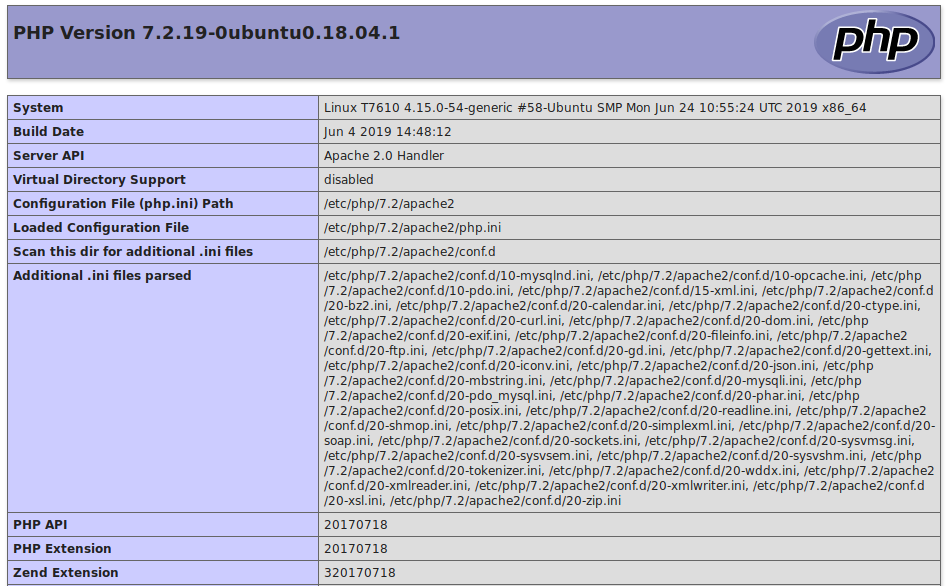
\includegraphics[width=1\linewidth]{phpinfo.png}
    \end{center}
  \end{figure}
\end{frame}

\subsection{And Finally...}
\begin{frame}{Enabling \texttt{PHP} for \texttt{user} directories}
  \begin{itemize}
    \item By default the \texttt{user directory} sites do not get access to \texttt{PHP} scripting.
    \item The scripting is disabled as part of the configuration of \texttt{PHP}.
    \item It can be enabled in the \texttt{php} config file.
  \end{itemize}
  \begin{tcolorbox}
    \begin{center}
      \scriptsize \texttt{/etc/apache2/mods-available/php7.2.conf}\\
      That's something for you to research in your own time!
    \end{center}
  \end{tcolorbox}
\end{frame}

\section*{Conclusion}
\begin{frame}{Conclusion}
  \begin{itemize}
    \item What is a Web Server?
    \item How do install \texttt{Apache}?
    \item What is a \texttt{Virtual} Websites?
    \item How does \texttt{Apache} Support Dynamic Scripting?
  \end{itemize}
\end{frame}

\end{document}


